% !TEX root = ../report.tex

\section{Key Drivers}
\label{sec:keydrivers}


Docker has the following key drivers
\begin{itemize}
	\item \req{kd}-- Portability
	\item \req{kd}-- Security
	\item \req{kd}-- Reliability
%	\item \req{kd}-- Compatibility
	%\item \req{kd}-- Maintainability
\end{itemize}
%
\subsection{Portability}
\label{subsec:kd-portability}
%
%Degree of effectiveness and efficiency with which a system, product or component can be transferred from one hardware, software or other operational or usage environment to another. This characteristic is composed of the following subcharacteristics:
%
%Adaptability. Degree to which a product or system can effectively and efficiently be adapted for different or evolving hardware, software or other operational or usage environments.
%Installability. Degree of effectiveness and efficiency with which a product or system can be successfully installed and/or uninstalled in a specified environment.
%Replaceability. Degree to which a product can replace another specified software product for the same purpose in the same environment.

%https://www.docker.com/
%Achieve agility and control for Development and IT Operations teams to build, ship, and run any app, anywhere

%https://github.com/docker/docker
% and are designed from the ground up with an application-centric design.”
%https://docs.docker.com/engine/installation/

Looking at Figure~\ref{fig:stakeholders-quality}, which visualizes the quality concerns of the stakholders, it is apparent that portability is the quality that is most desired among the stakeholders. One of the main features, if not the main feature of Docker, is to provide ``agility and control for Development and IT Operations teams to build, ship, and run any app, anywhere''\cite{dockermain}.\\
Docker wants the containers running the applications to be ``hardware-agnostic'' and ``platform-agnostic'' \cite{dockerrepo}, meaning that Docker containers do not know anything about the hardware, nor the platform it is run on, thus making it very portable. This allows developers to focus on the actual application, without having to worry about the underlying hardware or platform. The applications the developers create could then be run everywhere where docker is supported.\\
To provide this quality attribute, Docker is also focused on increasing the performance. To truly be able to replace applications, the docker containers must perform comparable to running the application natively, using a comparible amount of system resources. Running an application inside a VM makes it somewhat portable. However, if the VM can only be run on systems that can cope with the increased use of system resources, the portability is reduces significantly. By making the Docker containers small, yet having a high performance, the containers become usable by a wide variety of systems and are able to replace the need to use any virtual machines that would otherwise be used to achieve this level of 0portability\cite{dockerrepo}. IBM has researched and compared the performance of VM's and containers \cite{IBM-performance}. This research shows that the performance overhead of docker is indeed minimal, as is shown in table \ref{fig:ibm-dockerperforrmance}.

\begin{figure}[H]
\centering
\begin{center}
  \makebox[\textwidth]{%
	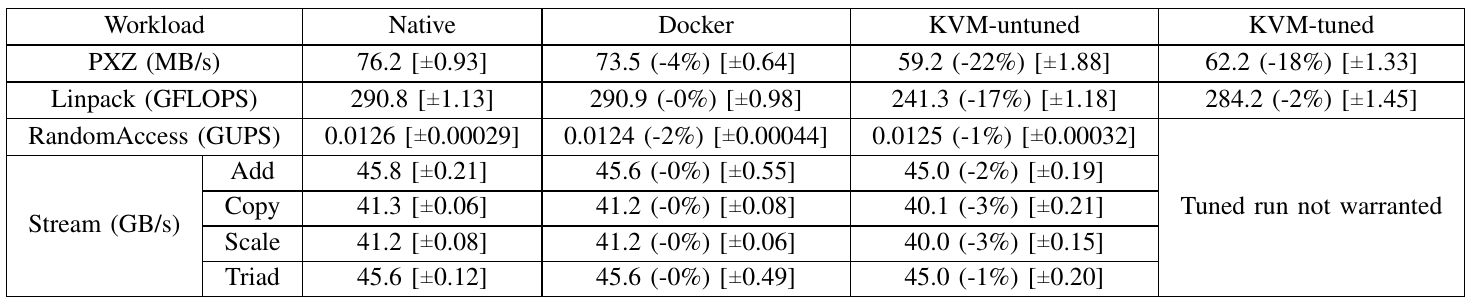
\includegraphics[width=0.9\paperwidth]{3-stakeholders/images/IBM-PerformanceCompare.png}}
\end{center}
\captionsource{Performance comparison results for PXZ, Linpack , Stream, and Random access. Each data point is the arithmetic mean of ten runs. Departure from native execution is show within parentheses ``()''. The standard deviation is shown within square brackets.}{\cite{IBM-performance}}%
\label{fig:ibm-dockerperforrmance}
\end{figure}

To increase the portability even more, docker provides a service to upload and share docker containers, making docker even more portable. This service is called the ``Docker hub'', which is a ``docker registry'' and will be discussed in \ref{subsec:dockerregistry}.

\subsection{Security}
The Docker daemon executes software inside containers and exposes an API. If somebody would gain unauthorized access to this API, this attacker would be capable of executing any program on the vulnerable host machine. Therefore, security is an important key driver for Docker. 

Additionally, since Docker does not use separated operating systems, but instead operating-system-level virtualization, the security and isolation of the containers is a serious concern if software inside the containers is not trusted. For example, for a cloud provider running containers for clients, isolation of these containers is an important aspect of the security, since clients should not be able to access data of other clients.


\subsection{Reliability}
The main function of a Docker container is to run a certain application. However, a system usually needs to run a set of different applications and it should not be the case that running these applications in Docker compromises the systems reliability.\\
Dependencies often lead to problems\cite{dockerrepo}, decreasing the reliability of software. The Docker files are text files containing a small set of instructions that will run an application. This means that the instructions needed to run an application are conveniently located in a single place, the Dockerfiles. This  allows viewing and the dependencies of all the different applications and making them easily maintainable.\\
Docker increases the reliability of the applications it runs, by increasing the testability of the containers and applications.\\
To make sure Docker itself stays reliable, it provides a test framework and test functions that thoroughly test the Docker software. \cite{dockertest}\\
% https://docs.docker.com/opensource/project/test-and-docs/
%
%makes systems and applications very maintainable.\\
%Dependencies of applications are centralized and easily manageable.\\
%Docker files are small text files, making it very share able. Instead of having to share an image of a VM, the docker file can be used to reuse an application or system anywhere.\\

%An application that is run on docker should not run slower and respond slower then if the application is not run in docker.\ign(natively) Database systems need to respond fast or anything that uses the database responds slow as well.\\
%The goal of a docker container is to run a certain application. However, a system usually needs to run a set of different applications and should not be the case that running these applications in docker compromises the system's resources.\\

%\subsection{Compatibility}
%The main goal of the docker project is to ``Build,Ship, and Run Any App, Anywhere'' \cite{dockermain}. To accomplish this, the docker containers need to be able to run on many different kinds of systems and platforms.\\
%Docker containers behave like a virtual machine and can easily be configured to communicate with each other.\\
%Docker also allows running the same application on multiple platforms. This allows the underlying operating system of an application to be changed, without compromising the system as a whole.